%%%%%%%%%%%%%%%%%%%%%%%%%%%%%%%%%%%%%%%%%%%%%%%%%%%%%%%%%%%%%%%%%%%%%%%%%%%%%
%% INÍCIO CAPÍTULO                                                         %%
%%%%%%%%%%%%%%%%%%%%%%%%%%%%%%%%%%%%%%%%%%%%%%%%%%%%%%%%%%%%%%%%%%%%%%%%%%%%%

\chapter{Análise de algoritmos de busca em árvores e tabelas de dispersão}
\label{cap:3:desenvolvimento}

\citacao{%
The greatest teacher, failure is.}
{Yoda}

\section{Definição formal do problema de busca}

O problema de busca, como apresentado no Capítulo \ref{cap:1:intro}, é um problema bastante recorrente na Computação.
Sua definição formal consiste em: \\

\textbf{Input: } Uma estrutura de $n$ dados $(d_1, d_2, d_3,\ldots, d_n)$ e um dado $x$ \\

\textbf{Output: } A localização do dado $x$ na estrutura $(d_1, d_2, d_3,\ldots, d_n)$. \\

Para este algoritmo, foram pensadas diversas soluções e estruturas de dados que facilitam o algoritmo 
e neste capítulo, será realizado o estudo e compreensão das mesmas. 
É importante perceber que, podemos aproximar a ordem de crescimento do algoritmo de ordenação
por inserção de forma bastante precisa utilizando as notações assintóticas, mas não é possível
determinar o tempo de execução para um número de entradas $n$ com muita precisão devido a aspectos
computacionais como:

\begin{itemize}
    \item Chaveamento e prioridade de processo no sistema operacional
    \item Tempo de execução de cada instrução do código compilado
    \item Velocidade de clock inconstante
\end{itemize}

\section{Busca em árvore não-ordenada} \label{cap:3:section:btree}

\subsection{Introdução}

O algoritmo de busca em árvore não-ordenada funciona de modo que, eu atravesse todos
nós da minha árvore até que eu ache o elemento $x$ que está sendo buscado, se isso acontece
é retornado o nó que contém $x$.

\subsection{Implementação}

A implementação do algoritmo de busca em árvore não-ordenada consiste em atravessar todos os
nós da esquerda e depois os nós da direita, se o elemento é encontrado, ele é retornado de forma
recursiva.

\begin{lstlisting}[style=CStyle]
BinaryNode * search(BinaryNode * root, int key) 
{
    if (root == NULL || root->data == key) {
        return root;
    }

    BinaryNode * found = search(root->left, key);
    if (found == NULL) {
        found = search(root->right, key);
    }

    return found;
}
\end{lstlisting}
            

Seu tempo de execução é na ordem da equação \ref{cap:3:eq:bTree}.

\begin{equation} \label{cap:3:eq:bTree}
    T(n) = O(n)
\end{equation}

\subsection{Resultados}

Para a implementação, foi obtido o gráfico \ref{cap:3:graph:bTree}:

\begin{figure}[h]
    \centering
    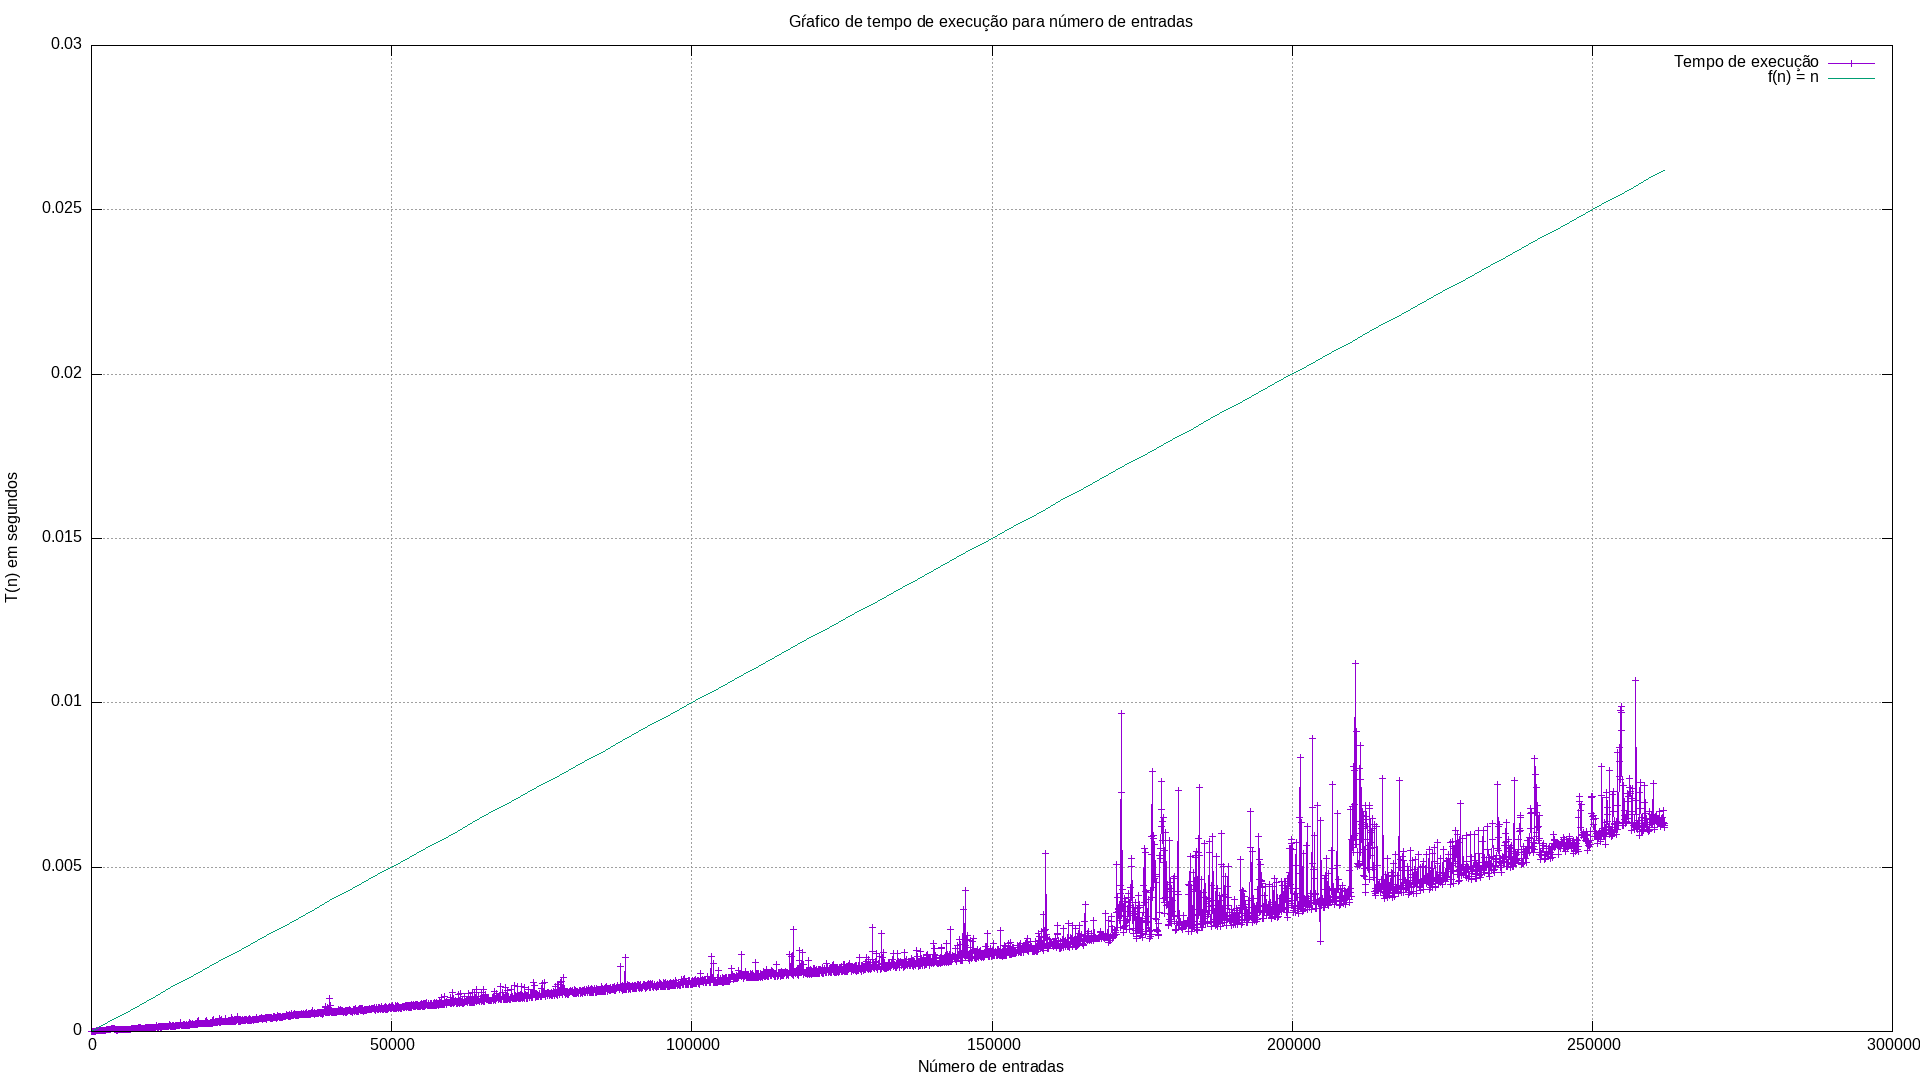
\includegraphics[width=\textwidth]{image/graphics/btree.png}
    \caption{Gráfico com tempo de execução do algoritmo de busca em árvore não-ordenada}
    \label{cap:3:graph:bTree}
\end{figure}

O gráfico obtido indica que:

\input{content/chapter/3/hashSearch}
\section{Busca em árvore binária de busca} \label{cap:3:section:bst}

\subsection{Introdução}

O algoritmo de busca em árvore binária de busca, funciona de modo que, vamos percorrer
a árvore, testando se o nó atual é maior ou menor que o elemento $x$, se for maior, tomamos
o caminho da esquerda, se for menor, tomamos o caminho da direita. Esse algoritmo pode ser implementado
porque a árvore binária de busca é uma estrutura que segue as seguintes proposições:

\begin{align*}
    NODE.PARENT \geq NODE.LEFT \\
    NODE.PARENT \leq NODE.RIGHT
\end{align*}

\subsection{Implementação}

A implementação do algoritmo de busca em árvore binária de busca funciona percorrendo
a árvore de forma organizada com as comparações do nó atual com o elemento $x$.

\begin{lstlisting}[style=CStyle]
Node * search(Node * root, int key) 
{
    if (root == NULL || root->data == key) {
        return root;
    }

    if (key < root->data) {
        return search(root->left, key);
    } else {
        return search(root->right, key);
    }
}
\end{lstlisting}
                    

Seu tempo de execução é na ordem da equação \ref{cap:3:eq:bst}.

\begin{equation} \label{cap:3:eq:bst}
    T(n) = O(\log n)
\end{equation}

\subsection{Resultados}

Para a implementação, foi obtido o gráfico \ref{cap:3:graph:bst}:

\begin{figure}[h]
    \centering
    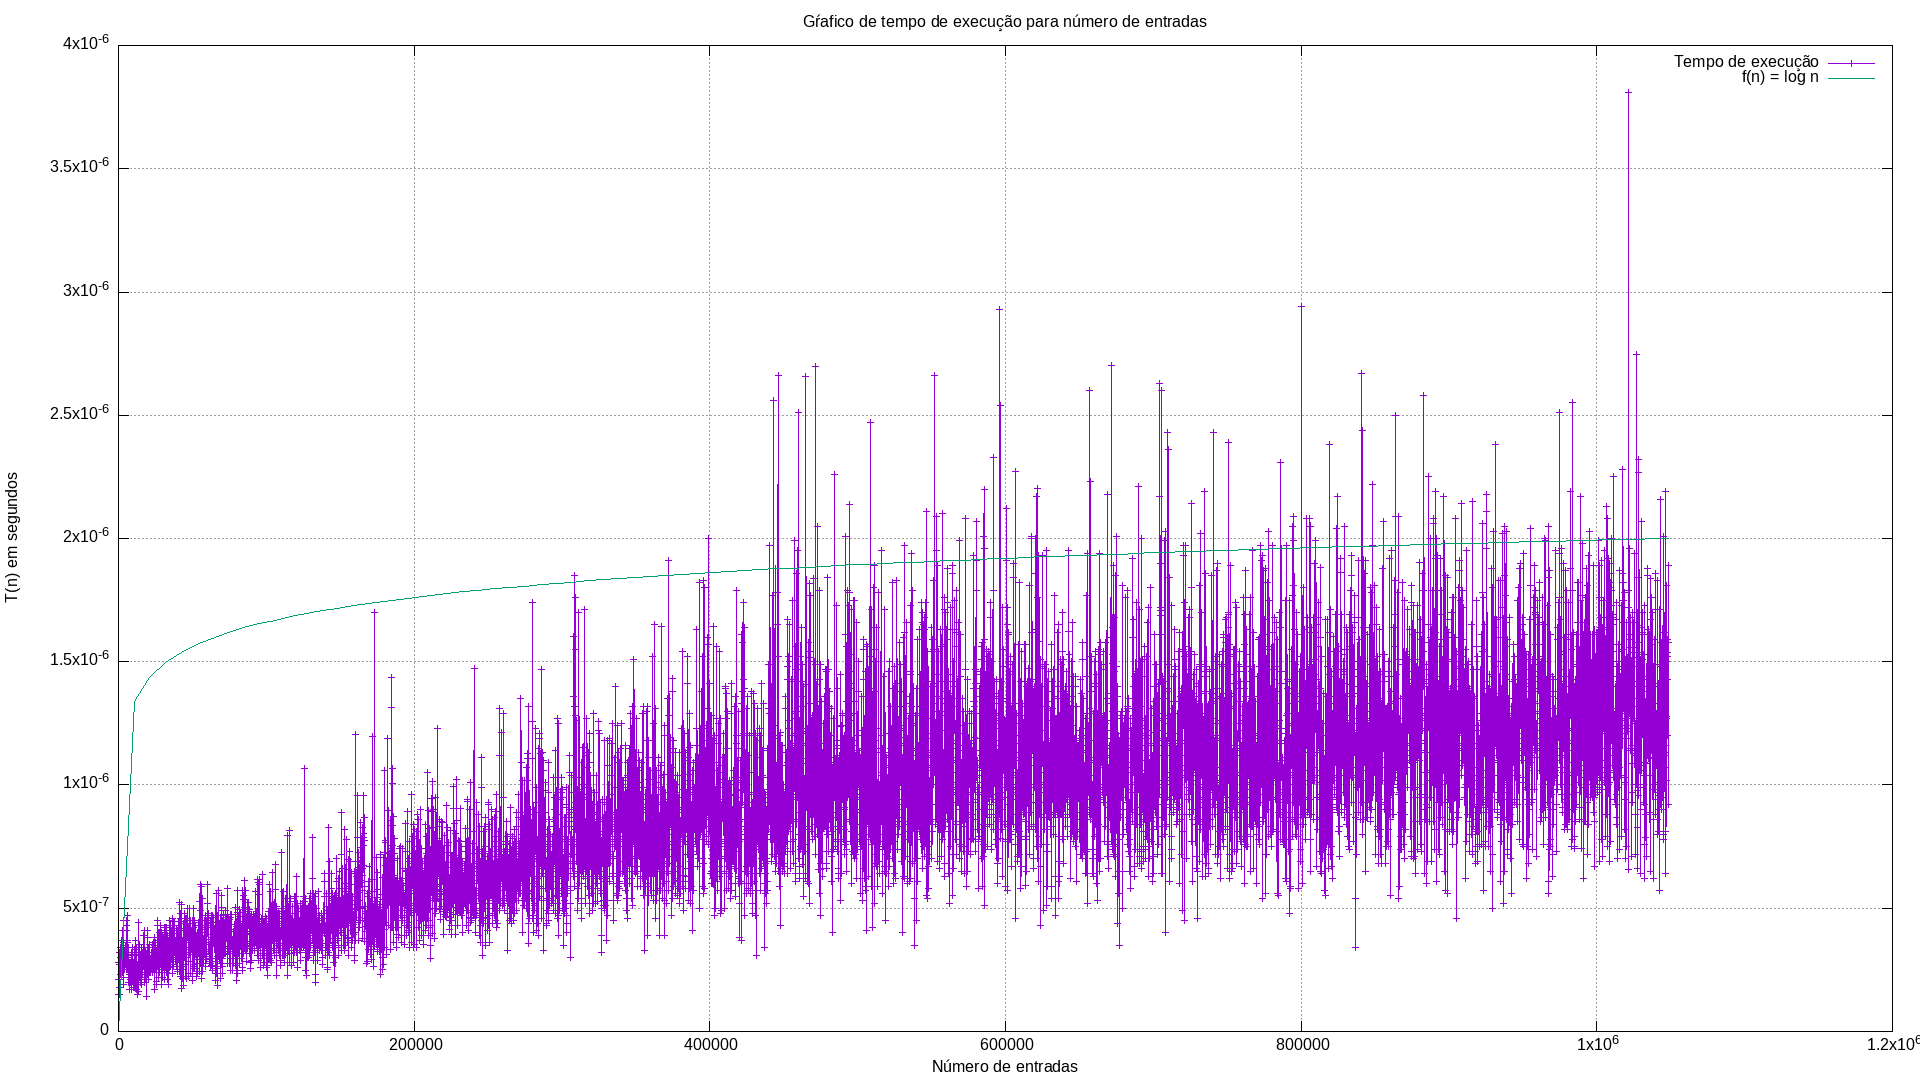
\includegraphics[width=\textwidth]{image/graphics/bst.png}
    \caption{Gráfico com tempo de execução do algoritmo de busca em árvore de busca binária}
    \label{cap:3:graph:bst}
\end{figure}

O gráfico obtido indica que:

\begin{enumerate}
    \item É compatível com a afirmação que $T(n) = O(\log n)$, já que, $O(\log n)$ é um limite superior.
    \item É um algoritmo muito rápido para buscar elementos em uma árvore pré-ordenada.
\end{enumerate}


%%%%%%%%%%%%%%%%%%%%%%%%%%%%%%%%%%%%%%%%%%%%%%%%%%%%%%%%%%%%%%%%%%%%%%%%%%%%%
%% FIM CAPÍTULO                                                            %%
%%%%%%%%%%%%%%%%%%%%%%%%%%%%%%%%%%%%%%%%%%%%%%%%%%%%%%%%%%%%%%%%%%%%%%%%%%%%%
